\chapter{RESULTS AND ANALYSIS}

\section{EEG Signal Acquisition Result}
Signals with lower amplitudes in the microvolt level were fed to the input of the instrumentation amplifier in order to simulate EEG signals. The signal at the output of the instrumentation amplifier designed using the AD620 showed no signs of distortion. The output signal proved to be stable enough to be processed in the next steps.
Thus, the amplification stage has shown itself to be effective enough to amplify low-level biopotential signals.

\section{High Pass Filter}
 
\begin{figure}[H]
	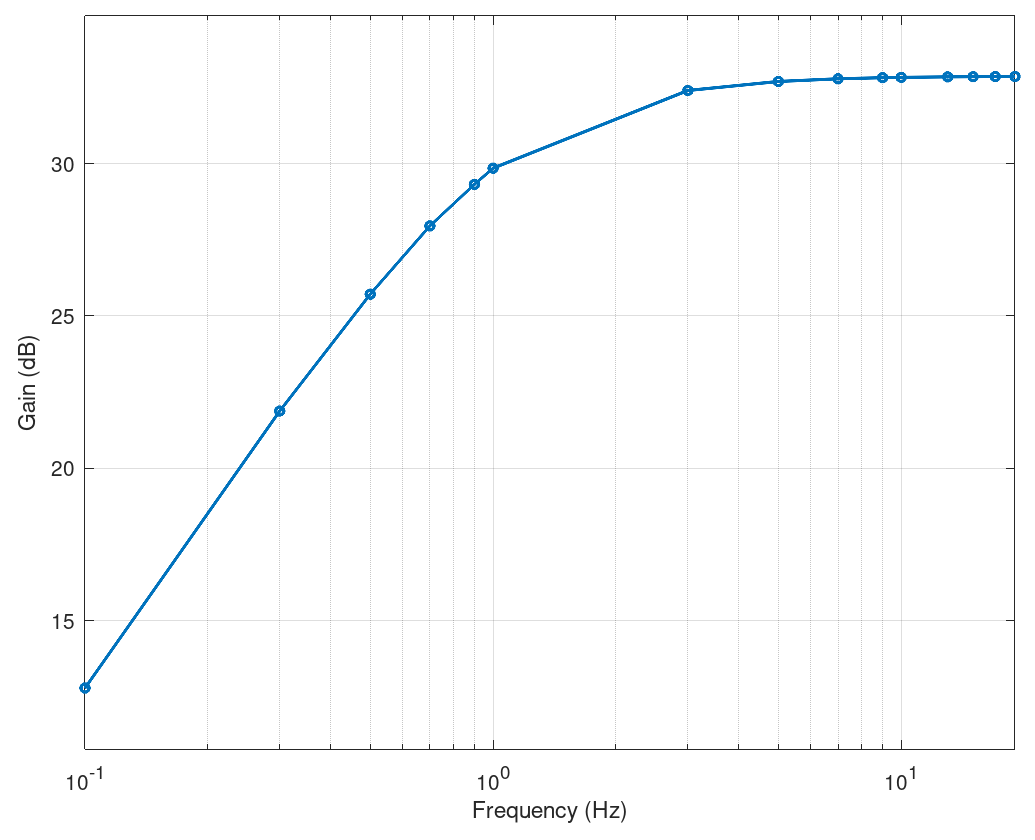
\includegraphics[width=\textwidth]{src/images/figures/highpass_plot.png}
	\caption{Bode plot of High Pass Filter's frequency response}
	\label{frequency_response_highpass}
\end{figure}

\section{Band Pass Filter}
\begin{figure}[H]
	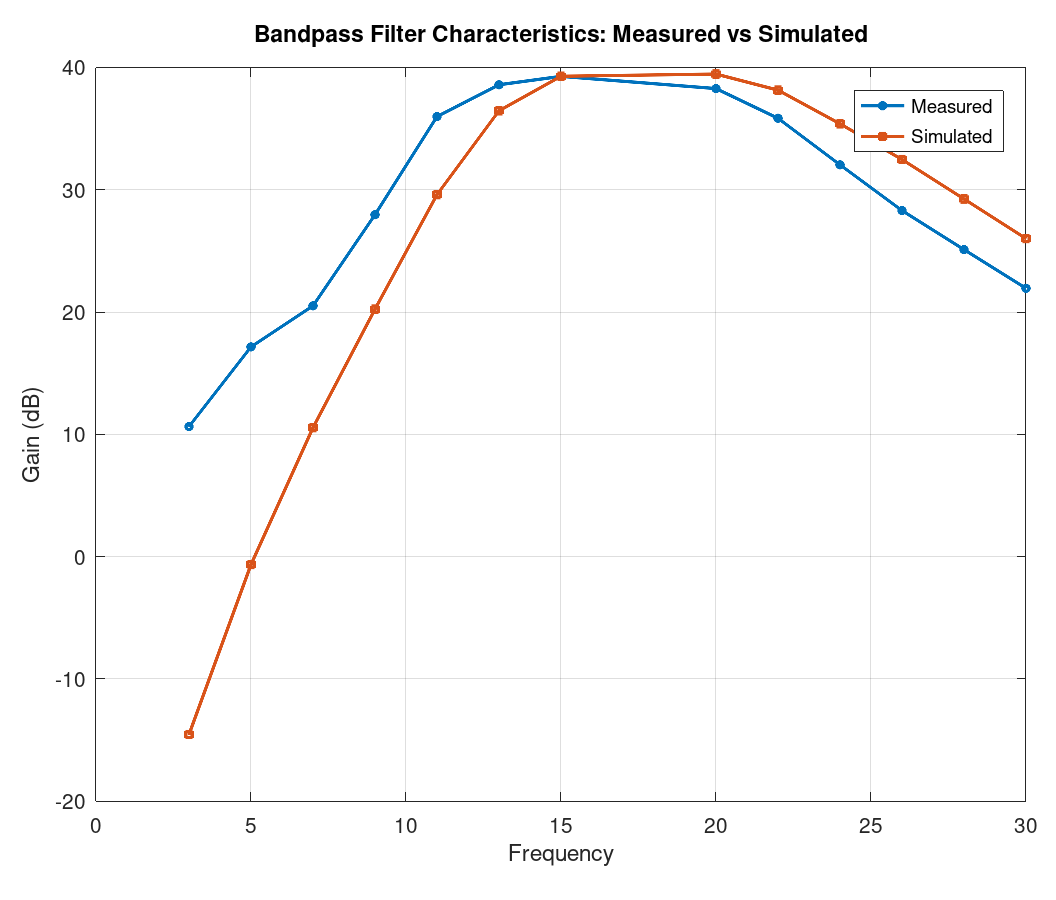
\includegraphics[width=\textwidth]{src/images/figures/bandpass_compare.png}
	\caption{Frequency Response of Band Pass Filter}
	\label{bandpass_compare}
\end{figure}

\section{FFT of Recieved Signal}
\begin{figure}[H]
	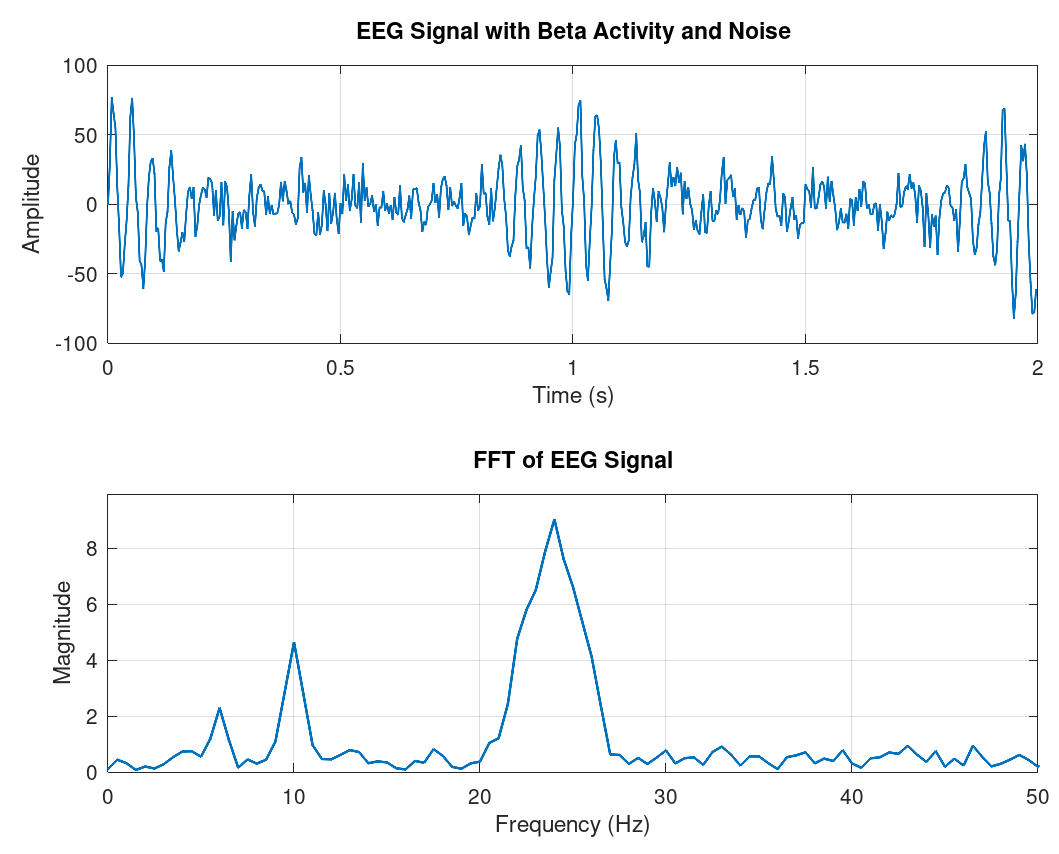
\includegraphics[width=\textwidth]{src/images/figures/betawaves.png}
	\caption{FFT plot of recieved signal}
	\label{betawaves}
\end{figure}

The filtered signal showed significant reduction in noise components, resulting in a cleaner waveform suitable for frequency analysis.

\section{Frequency Domain Analysis Using FFT}
FFT was used on the filtered signal in order to transform the signal from the time domain into the frequency domain. The FFT result showed prominent frequency peaks representing the frequency of the input signal from the function generator.

Upon setting the input signal frequency in the beta band range (12-30 Hz), a pronounced peak was seen in the FFT graph in the beta band range. This proves that the system can detect certain EEG frequency bands using frequency domain analysis.

\section{Confusion Matrix}
\begin{figure}[H]
	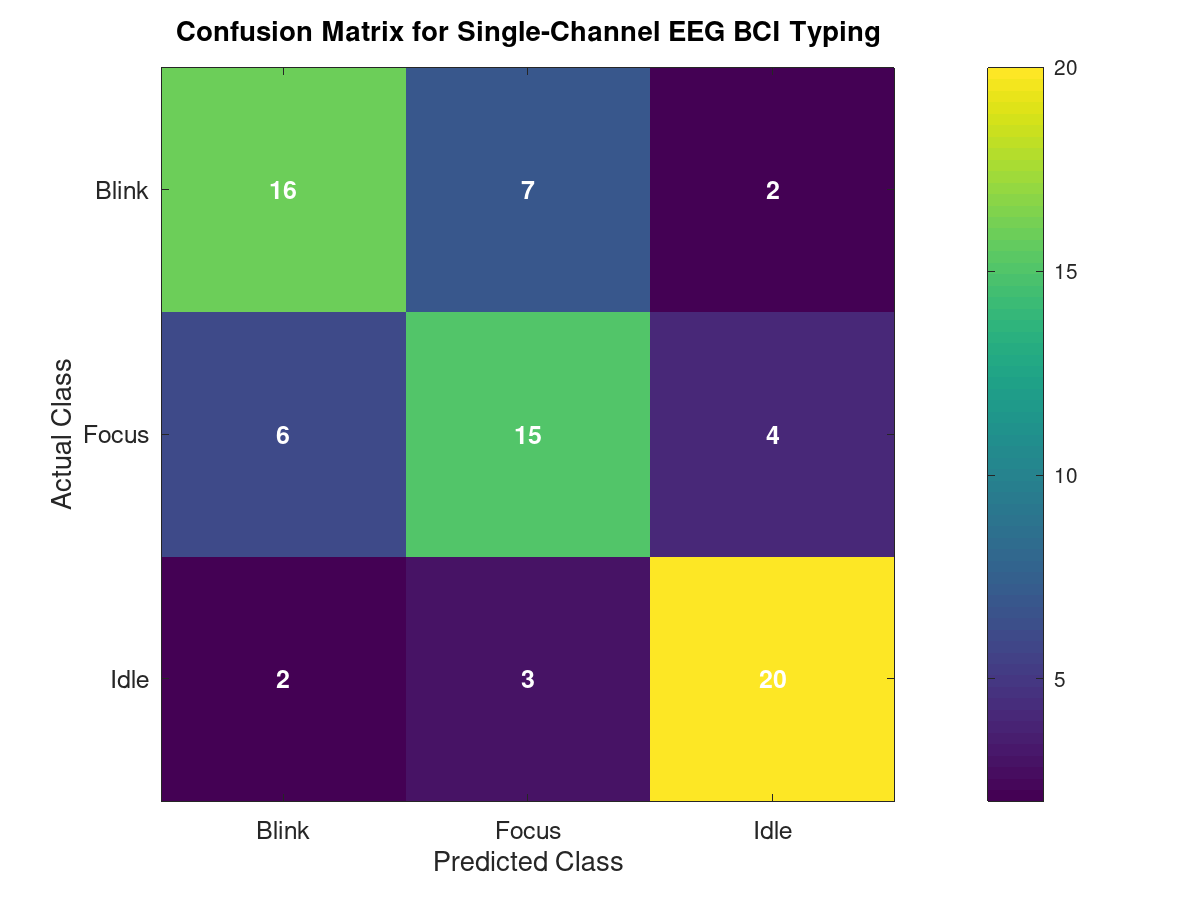
\includegraphics[width=\textwidth]{src/images/figures/confusion.png}
	\caption{Confusion Matrix}
	\label{confusion}
\end{figure}

This confusion matrix was used to analyze the classification ability of single-channel EEG-based BCI typing system in distinguishing three states: blink, focus and idle. Rows correspond to the actual classes, whereas columns denote the classes assigned by the system. The numbers along the diagonal represent the correct classifications. In other words, the system identified 16 blinks, 15 focuses and 20 idles out of 25 trials of each class respectively. Thus, the total accuracy equals to 68\%. These results prove that the system is capable of detecting user intentions at the most general level. Nevertheless, it should be noted that the performance was different for each particular class.

One may observe the main issue represented in the confusion matrix, namely the confusion between blink and focus. More specifically, there were 7 cases when blink was identified as focus and 6 cases when focus was confused with blink. In other words, these types of mistakes comprised the major source of errors in the system. One of the reasons behind this problem was that blink and focus were measured from the same channel of EEG. The fact that only one channel was used made it rather difficult to distinguish between two types of activity. A blink usually causes significant signal shift, however, focus may also lead to such changes, particularly if the user makes some slight movements with eyes, changes forehead tension and produces muscular activity while concentrating. Consequently, the system managed to understand that some intentional activity occurred, but failed to determine whether it was blink or focus.

As for the results achieved for the idle class, they were rather good, i.e. 20 correct identifications out of 25. This may be explained by the fact that idle state is more stable and close to the baseline signal than other two types of activity. Nevertheless, several cases of incorrect classification were also observed for this type. They might be caused by noise, unintentional movements of eyes and some signal shifts which had nothing in common with any commands. As for the worst results obtained for focus, they are quite understandable. It is much easier to identify blink than focus since blink lasts for a rather short period, whereas focus refers to some kind of mental state changing very slowly.


